% Dale's affiliation
% insert missing reference to Katayama and Kim (2012) cited in footnote 13.
% fix capitalization in bibliography



\newcommand{\footnoteSS}[1]{\footnote{
\renewcommand{\baselinestretch}{1.0} \footnotesize \setlength{\oddsidemargin}{-0.4in}
\setlength{\evensidemargin}{-0.4in} \setlength{\textwidth}{7.2in}
#1}}


\documentclass[12pt,fleqn]{article}
%%%%%%%%%%%%%%%%%%%%%%%%%%%%%%%%%%%%%%%%%%%%%%%%%%%%%%%%%%%%%%%%%%%%%%%%%%%%%%%%%%%%%%%%%%%%%%%%%%%%%%%%%%%%%%%%%%%%%%%%%%%%%%%%%%%%%%%%%%%%%%%%%%%%%%%%%%%%%%%%%%%%%%%%%%%%%%%%%%%%%%%%%%%%%%%%%%%%%%%%%%%%%%%%%%%%%%%%%%%%%%%%%%%%%%%%%%%%%%%%%%%%%%%%%%%%
\usepackage{amsmath}
\usepackage{slashed}
\usepackage{amssymb}
\usepackage{graphicx}
\usepackage{chicago}

\setcounter{MaxMatrixCols}{10}
%TCIDATA{OutputFilter=Latex.dll}
%TCIDATA{Version=5.50.0.2960}
%TCIDATA{<META NAME="SaveForMode" CONTENT="1">}
%TCIDATA{BibliographyScheme=BibTeX}
%TCIDATA{LastRevised=Friday, October 07, 2011 15:01:21}
%TCIDATA{<META NAME="GraphicsSave" CONTENT="32">}

\setlength{\paperwidth}{8.5in} \setlength{\paperheight}{11.0in}
\setlength{\topmargin}{0.0in} \setlength{\headheight}{0.4in}
\setlength{\headsep}{0.0in} \setlength{\textwidth}{7.2in}
\setlength{\textheight}{8.5in} \setlength{\oddsidemargin}{0.0in}
\setlength{\oddsidemargin}{-0.4in}
\setlength{\evensidemargin}{-0.4in}
\renewcommand{\baselinestretch}{1.5}
\renewcommand{\textfraction}{0.33}

\input{tcilatex}

\begin{document}


\renewcommand{\baselinestretch}{1.0}

\begin{center}
{\normalsize \thispagestyle{empty} }

{\normalsize \medskip }

%{\normalsize {\Large Do the Sources of Sector-Specific Shocks Matter for Aggregate Outcomes?$^{*}$%
%} \medskip }

{\normalsize {\Large Modeling Investment-Sector Efficiency Shocks: \\[0pt]
 When Does Disaggregation Matter?$^{*}$} \medskip }

{\normalsize \bigskip \bigskip }

{\normalsize Luca Guerrieri, Dale Henderson, and Jinill Kim }

{\normalsize \bigskip \bigskip }

{This Draft: February, 2013 }

{\normalsize \bigskip }
\end{center}

{\normalsize \bigskip }

\abstract{The most straightforward way to analyze investment-sector productivity developments is to construct a two-sector model with a sector-specific productivity shock. An often used modeling shortcut accounts for such developments using a one-sector model with shocks to the efficiency of investment in a capital accumulation equation. This shortcut is theoretically
justified when some stringent conditions are satisfied. Using a
two-sector model, we consider the implications of relaxing several
of the conditions that are at odds with the U.S. Input-Output
Tables, including equal factor shares across sectors.  The
effects of productivity shocks to an investment-producing sector of
our two-sector model differ from those of efficiency shocks to investment in a one-sector
model. Notably, expansionary productivity shocks boost consumption at all horizons, while expansionary efficiency shocks reduce consumption initially.}

{\normalsize \vspace{1.0cm} }

{\normalsize \noindent \textbf{Keywords}: DSGE Models, Multi-Factor
Productivity Shocks, Marginal Efficiency of Investment Shocks, Investment-Specific Technology Shocks \vspace{1cm} }

{\normalsize \noindent \textbf{JEL Classification}: E13, E32 }

{\normalsize \vspace{1cm} }

\renewcommand{\baselinestretch}{1} {\footnotesize \noindent }

{\footnotesize \textbf{\ Affiliation and contact information}: Luca
Guerrieri, Federal Reserve Board, telephone (202) 452 2550, email
luca.guerrieri@frb.gov; Dale Henderson, Cardiff University, email
dale.henderson@rcn.com; Jinill Kim, Korea University, email
jk9n@hotmail.com. }

{\footnotesize \vspace{2cm} }

{\footnotesize \noindent $^{*}$ Previous drafts of this paper were
circulated under the title ``Interpreting Investment-Specific Technology
Shocks'' and ``Sector-Specific Productivity Shocks and Aggregate Outcomes: What You Put In Affects What You Get Out.'' The views expressed in this paper are solely the responsibility of
the authors and should not be interpreted as reflecting the views of the
Board of Governors of the Federal Reserve System or of any other person
associated with the Federal Reserve System.  }

\clearpage \renewcommand{\baselinestretch}{1.5} \normalsize

\section{\protect\normalsize Introduction}

In post-WWII U.S. data, the relative price of investment has a downward trend and varies over the cycle. Moreover, investment-sector productivity developments have been identified as a primary driver of the economic boom of the late 1990s.\footnoteSS{For instance, see \citeN{jorgenson2001}.} Perhaps the most
straightforward way to account for investment-sector productivity developments is to construct a two-sector
model with investment-sector multi-factor productivity (MFP) shocks. However, the more frequently used approach relies on shocks to the marginal efficiency of investment (MEI) in a capital accumulation equation of a one sector model.\footnoteSS{\citeN{greenwood1988} and Greenwood, Hercowitz, and Krusell (1997, 2000) used a one-sector model with a shock in the capital accumulation equation
to distinguish equipment investment from other final-use categories. Our choice of dubbing this shock ``MEI'' follows Greenwood, Hercowitz, and Huffman (1988), whereas  Greenwood, Hercowitz, and Krusell (1997, 2000) referred to the same shock as an ``investment-specific technology shock,'' a choice justified under certain restrictive conditions for our extended two-sector model.}
In fact, MEI shocks have become the leading candidate explanation for post-war business
cycle fluctuations.\footnoteSS{%
Prominent examples are \shortciteN{fisher2006}, \shortciteN{smets2007}, \shortciteN{justiniano2008}, and \shortciteN{papanikolaou2011}.}
The focus of this paper is on
investment-sector efficiency shocks, their effects, and the implications of capturing them with MFP shocks or with MEI shocks. As we show, alternative ways of accounting for sectoral productivity developments lead to
differences in both qualitative and quantitative outcomes for aggregate
variables.

\shortciteN{greenwood1997} pioneered the MEI approach. \shortciteN{greenwood2000} show that their one-sector model is a special case of a
model with two sectors, one that produces a good used only for equipment
investment and another that produces a good used for both consumption and
structures investment. Under certain conditions, an MEI shock to the equipment accumulation equation of their one-sector model is equivalent for aggregate variables
to an MFP shock to equipment production in the
two-sector model. This ``aggregate equivalence'' result provides a
basis for interpreting MEI shocks as MFP shocks.

It may come as no surprise that the conditions for aggregate equivalence are
quite restrictive. Capital is taken to be perfectly mobile between sectors
and no allowance is made for costs of adjusting investment. We show that the
conditions also entail a production structure that differs significantly
from the one implied by the U.S. Input-Output (IO) Tables. For instance, the
conditions require the same factor shares across sectors, while we show that
factor shares are quite different across sectors. In a paper with a focus
different from ours, \shortciteN{basu2010} also show that the structure of U.S.
production implies different factor shares across sectors.\footnoteSS{%
Their main contribution is to develop a new method of estimating
sector-specific technology shocks.}

We show how reasonable departures from the restrictive conditions for equivalence
affect the aggregate outcomes of both sectoral MFP shocks and MEI shocks. Our
model has two production sectors, a machinery-producing sector and its complement, a non-machinery-producing sector, and is calibrated to the U.S. IO Tables and
other sectoral statistics.\footnoteSS{%
One of the first papers to emphasize the importance of the input-output
structure for the business cycle is \shortciteN{long1983}. More recent
contributions include \shortciteN{hornstein1997} and \shortciteN{edge2008}.} In this
model, MFP increases in the machinery-producing sector have effects that are
qualitatively different from MEI increases in a one-sector model, even
though the models are calibrated to match the same aggregate features
whenever possible. One important difference is that with MFP shocks,
consumption is boosted at all horizons, while with MEI shocks consumption is
reduced initially.\footnoteSS{%
In related work, \shortciteN{Swanson2006} showed that MFP shocks at the sectoral
level in a multi-sector model can lead to different aggregate implications
from those of MFP shocks in a one-sector model.}

Following the empirical support for the importance of investment shocks provided by \shortciteN{fisher2006}, \shortciteN{smets2007}, and \shortciteN{justiniano2008}, a growing number of papers that estimate dynamic stochastic general equilibrium (DSGE) models have included such shocks and found them to be a major driver of business cycle
fluctuations. However, these studies struggle with the problem that if MEI shocks are
prominent, they may cause the unconditional correlation between investment and consumption
to be counterfactually negative. MFP shocks
in the machinery sector, while sharing many features with MEI shocks, can resolve this
incongruence.\footnoteSS{In \citeN{guerrieri2010} we use Monte Carlo methods to show that MFP shocks in our two-sector model are much more likely than MEI shocks in a one-sector model to produce the strong positive correlation between consumption and investment found in the data. }

There are other ways of generating comovement between
consumption and investment. A good overview of the literature on
comovement is provided by \shortciteN{christiano98}.\footnoteSS{In an
open economy setting, \shortciteN{raffo2010} shows that MEI shocks may
help generate improvements in the terms of trade in periods of
economic expansion.} The mechanism suggested by
\shortciteN{greenwood2000} revolves around variable capacity
utilization for capital. \shortciteN{christiano2008} point to strong
consumption habits and investment adjustment costs as a mechanism
for generating comovement. \shortciteN{eusepi2008},
\shortciteN{jaimovich2009}, \shortciteN{furlanetto2010},  and
\shortciteN{papanikolaou2011} focus on departures from utility
functions that are additively separable in consumption and leisure
to generate comovement. While focusing on different issues,
\shortciteN{schmitt2011} offer yet another possible mechanism for
generating co-movement: correlated shocks. They notice that MFP
series from aggregate growth accounting exercises and the relative
price of equipment investment are co-integrated and reconcile this
finding with co-integrated neutral MFP and MEI shocks.

Our approach is different in several ways. We do not
have to introduce variable capacity utilization of factor inputs. The specification of preferences we consider is time separable.
We obtain comovement while abstracting from consumption habits and the labor-leisure choice
altogether. Although we allow for investment
adjustment costs, our two-sector model does not rely on such costs
to generate comovement. Finally, given that the conditions for
aggregate equivalence fail in our two-sector model, it is possible to find
that aggregate MFP measures and the relative price of equipment
investment are cointegrated even when maintaining the hypothesis
of orthogonal shocks across sectors.

\section{\protect\normalsize The model}

Our approach to the analysis of productivity changes is a
combination of the growth-accounting approach based on industrial
breakdowns---in the tradition of \shortciteN{solow1957} and \shortciteN{jorgenson1966}%
---and the approach based on final-use breakdowns typical of DSGE models.\footnoteSS{We refer to \textquotedblleft production
sectors\textquotedblright rather than \textquotedblleft
industries\textquotedblright because the former terminology is more common
in the DSGE literature to which our paper is somewhat more closely related.}

Our two-sector model has some similarities to the one posited
by \shortciteN{greenwood2000}. Both models have two production
sectors and the same three final goods (equipment investment, consumption,
and structures investment). However, our model emobodies three extensions. The first
extension is that the outputs of both the machinery ($M$) and non-machinery ($N$) sectors are used in
\textquotedblleft assembling\textquotedblright\ all three final goods.  For example, equipment investment is
assembled using machines from the $M$ sector and distribution services from
the $N$ sector. Thus, the structure of our economy differs from that in \shortciteN{greenwood2000}
except in the limiting case of ``complete specialization in assembly'' in
which $M$ output is used only in the assembly of equipment and $N$ output is
used only in the assembly of consumption and structures. In this limiting
case, the machinery sector could just as well be referred to as the
equipment sector, as it is in \shortciteN{greenwood2000}.

The other two extensions are additions of two types of real
rigidities. First, as has become common in DSGE models, we allow for costs of adjusting investment.%
\footnoteSS{%
Investment adjustment costs are not a part of the model developed by %
\shortciteN{greenwood1997} and \shortciteN{greenwood2000}, but are a common
ingredient of models developed subsequently that also incorporate
MEI shocks.} This extension enables us to consider conditions for
equivalence under alternative specifications of these costs.
Second, we allow for costs of adapting capital suitable for one
sector for use in the other. This extension makes it possible for
us to consider the case in which capital stocks are predetermined
not only at the aggregate level but also essentially predetermined at the sectoral level.\footnoteSS{\shortciteN{ramey1998}
document the high costs of reallocating capital across sectors. \shortciteN{greenwood1997} abstract from adjustment costs of capital altogether. \shortciteN{greenwood2000} include sector-specific costs of adjusting capital over time, but continue to allow for the costless reallocation of capital across sectors within a period.}

\subsection{\protect\normalsize Production sectors}

{\normalsize Our two production sectors, the $M$ and $N$ sectors, comprise perfectly competitive firms. Consider the
representative firm in sector $i$ (where $i\in \{M,N\})$ in period $s$. It
hires labor ($L_{is}$) from households at a wage $\left( W_{s}\right) $ that
is same for both sectors because labor is perfectly mobile between sectors.
It also rents two types of capital from households: equipment capital ($%
K_{is}^{E}$) and structures capital $\left( K_{is}^{S}\right) $ at rentals ($%
R_{is}^{E}$ and $R_{is}^{S}$) that are sector-specific when it is costly
to reallocate capital. The firm minimizes the unit cost of producing a given
number of physical units of its sector's output ($Y_{is}$) subject to a
sector-specific Cobb-Douglas production function:
\begin{equation}
Y_{is}=\left( L_{is}\right) ^{1-\alpha _{i}^{E}-\alpha _{i}^{S}}\left(
K_{is}^{E}\right) ^{\alpha _{i}^{E}}\left( K_{is}^{S}\right) ^{\alpha
_{i}^{S}}.  \label{technology}
\end{equation}%
The factor shares for the two types of capital are $\alpha _{i}^{E}$ and $%
\alpha _{i}^{S}$. }

{\normalsize
%There is a multi-factor productivity (MFP) process $\tilde{A}_s $
%which determines the efficiency units generated by physical
%machinery output ($Y_{Ms}^{A}=\tilde{A}_s^{1-\alpha_M^E-\alpha_M^S} Y_{Ms}$). For example, for computers $%
%Y_{Ms}$ can be thought as the number of computers produced, and
%$Y_{Ms}^{A}$ as the computing power generated by these computers.
%The definition of $Y_{Ms}^{A}$ could be combined with Equation
%(\ref{technology}), and the term $\tilde{A}_s$ could then be
%interpreted as labor-augmenting technology. However, we find it
%convenient to account separately for physical and efficiency units
%when comparing sectoral MFP shocks with MEI shocks. To simplify the
%notation, define the MFP shock $A_s$ such that
%$A_s=\tilde{A}_s^{1-\alpha_M^E-\alpha_M^S}$.
}

{\normalsize There is a multi-factor productivity (MFP) process $A_s $ which
determines the efficiency units generated by physical machinery output ($%
Y_{Ms}^{A}=A_s Y_{Ms}$).\footnoteSS{%
Note that we do not consider MFP shocks to the non-machinery sector.}
For example, for computers $Y_{Ms}$ can be thought
as the number of computers produced, and $Y_{Ms}^{A}$ as the computing power
generated by these computers. We find it convenient to account separately
for physical and efficiency units when comparing sectoral MFP shocks with
MEI shocks. }

{\normalsize Since it is competitive and there are constant returns to
scale, the firm ends up selling at a price equal to unit cost. Let $P_{is}$
represent the factor cost of a unit of physical output~$i.$\footnoteSS{%
For example, $P_{M}$ is the multiplier in the Lagrangian expression ($%
\mathcal{L}_{M}$ ) used to the minimize costs of producing a given physical
quantity $Y_{M}$:%
\begin{equation}
\mathcal{L}_{M}=WN_{M}+R_{M}^{E}K_{M}^{E}+R_{M}^{S}K_{M}^{S}+P_{M}\left\{
Y_{M}-\left( L_{M}\right) ^{1-\alpha _{N}^{E}-\alpha _{N}^{S}}\left(
K_{M}^{E}\right) ^{\alpha _{N}^{E}}\left( K_{M}^{S}\right) ^{\alpha
_{N}^{S}}\right\} ,  \notag
\end{equation}%
where time subscripts have been omitted for simplicity.} We assume that the $%
N$ good is the numeraire, so $P_{Ns}=1$. The factor cost of a physical unit
of machinery is $P_{Ms}$ and the cost of an efficiency unit of machinery is $%
P_{Ms}^{A}=\frac{P_{Ms}}{A_s}$ so that%
\begin{equation}
P_{Ms}Y_{Ms}=\left( \frac{P_{Ms}}{A_s}\right) A_s
Y_{Ms}=P_{Ms}^{A}Y_{Ms}^{A}.  \label{Mvalue}
\end{equation}%
}

\subsection{\protect\normalsize Final goods}

{\normalsize There are three final goods: a consumption good ($C_{s}$) and
two investment goods, one ($J_{s}^{E}$) used for gross investment in $E$
capital stocks and the other ($J_{s}^{S}$) used for gross investment in $S$
capital stocks. These goods are assembled by perfectly competitive final
goods firms that use as inputs the outputs of the two production sectors,
and these final goods are measured in efficiency units. When we find it
expedient for the exposition, we us an upper bar to denote final goods
measured in physical units. }

{\normalsize The assembly function for $C_{s}$ is a constant elasticity of
substitution (CES) function of the two consumption inputs, efficiency units
of $M$ goods ($A_sC_{Ms}$) along with\ $N$ goods ($C_{Ns}$):
\begin{equation}
C_{s}=\left[ \phi _{M}^{C}\left( \frac{A_s C_{Ms}}{\phi _{M}^{C}}\right) ^{%
\frac{\sigma _{C}-1}{\sigma _{C}}}+\phi _{N}^{C}\left( \frac{C_{Ns}}{\phi
_{N}^{C}}\right) ^{\frac{\sigma _{C}-1}{\sigma _{C}}}\right] ^{\frac{\sigma
_{C}}{\sigma _{C}-1}},
\end{equation}
where $\phi _{M}^{C}$ and $\phi _{N}^{C}$ are the weights for $M$ and $N$
goods, and $\sigma _{C}$ is the elasticity of substitution between $M$ and $%
N $ goods in the assembly of $C_{s}$. }

{\normalsize The assembly functions for $J_{s}^{E}$ and $J_{s}^{S}$ are CES
functions of the two investment inputs, efficiency units of $M$ goods ($%
A_sI_{Ms}^{E}$, $A_sI_{Ms}^{S}$) along with $N$ goods ($I_{Ns}^{E}$, $%
I_{Ns}^{S}$):
\begin{equation}
J_{s}^{E}=\left[ \phi _{M}^{E}\left( \frac{A_s I_{Ms}^{E}}{\phi _{M}^{E}}%
\right) ^{\frac{\sigma _{E}-1}{\sigma _{E}}}+\phi _{N}^{E}\left( \frac{%
I_{Ns}^{E}}{\phi _{N}^{E}}\right) ^{\frac{\sigma _{E}-1}{\sigma E}}\right] ^{%
\frac{\sigma _{E}}{\sigma _{E}-1}},  \label{equipment assembly}
\end{equation}%
\begin{equation}
J_{s}^{S}=\left[ \phi _{M}^{S}\left( \frac{A_sI_{Ms}^{S}}{\phi _{M}^{S}}%
\right) ^{\frac{\sigma _{S}-1}{\sigma _{S}}}+\phi _{N}^{S}\left( \frac{%
I_{Ns}^{S}}{\phi _{N}^{S}}\right) ^{\frac{\sigma _{S}-1}{\sigma _{S}}}\right]
^{\frac{\sigma _{S}}{\sigma _{S}-1}},
\end{equation}%
where $\phi _{M}^{E},\phi _{N}^{E},\phi _{M}^{S}$ and $\phi _{N}^{S}$ are
the weights given to $M$ and $N$ goods, and $\sigma _{S}$ and $\sigma _{E}$
are the elasticities of substitution between $M$ and $N$ goods.  }

{\normalsize The assembly firms minimize the unit cost of producing
efficiency units of consumption, equipment, and structures.\footnoteSS{%
For example, $P^{J^{E}}$, is the multiplier in the Lagrangian expression ($%
\mathcal{L}_{J^{E}}$ ) used to the minimize costs of producing a given
quantity $J^{E}$:%
\begin{equation*}
\mathcal{L}_{J^{E}}=P_{M}I_{M}^{E}+I_{N}^{E}+P^{J^{E}}\left\{ J^{E}-\left[
\phi _{M}^{E}\left( \frac{A_sI_{M}^{E}}{\phi _{M}^{E}}\right) ^{\frac{\sigma
_{E}-1}{\sigma _{E}}}+\phi _{N}^{E}\left( \frac{I_{N}^{E}}{\phi _{N}^{E}}%
\right) ^{\frac{\sigma _{E}-1}{\sigma E}}\right] ^{\frac{\sigma _{E}}{\sigma
_{E}-1}}\right\},
\end{equation*}%
where time subscripts have been omitted for simplicity.} Because they are
perfectly competitive, firms end up selling final goods at prices that are
equal to these costs and that are indicated by $P_{s}^{C}$, $P_{s}^{J^{E}}$,
and $P_{s}^{J^{S}}$. We assume that the assembly functions for both $C_{s}$
and $J_{s}^{S}$ are $N$-intensive relative to the function for $J_{s}^{E}$. }

{\normalsize There is a shock $Z_s$ to the marginal efficiency of investment (MEI) which further enhances the efficiency of $J_{s}^{E}$, the
efficiency unit of equipment assembled using $M$ and $N$ inputs. The final
total amount of equipment efficiency units is given by $Z_s J_{s}^{E}$ and
the all-in unit cost is $\frac{P_{s}^{J^{E}}}{Z_s}$ so that%
\begin{equation}
P_{s}^{J^{E}}J_{s}^{E}=\left( \frac{P_{s}^{J^{E}}}{Z_s}\right) Z_sJ_{s}^{E}.
\end{equation}%
For example, the expressions $Z_sJ_{s}^{E}$ and $\left( \frac{P_{s}^{J^{E}}}{%
Z_s}\right)$ in the model are analogous to the measures of computer output
and the price of computer output in the NIPA. }

{\normalsize We sometimes refer to the case of \textquotedblleft partial
specialization\textquotedblright\ in assembly. Under partial specialization,
the assembly functions for $C$ and $J^{S}$ depend only on the $N$ good:
\begin{equation}
C_{s}=C_{Ns},\qquad J_{s}^{S}=I_{Ns}^{S},\qquad
Y_{Ns}=C_{Ns}+I_{Ns}^{S}+I_{Ns}^{E},
\end{equation}%
and the assembly function for total efficiency units of equipment
investment, $Z_sJ^{E}_s$, is Cobb-Douglas:
\begin{eqnarray}
Z_sJ_{s}^{E} &=& Z_s\left( A_sI_{Ms}^{E}\right) ^{\phi _{M}^{E}}\left(
I_{Ns}^{E}\right) ^{\phi _{N}^{E}}=Z_s\left( A_s\right) ^{\phi
_{M}^{E}}\left( I_{Ms}^{E}\right) ^{\phi _{M}^{E}}\left( I_{Ns}^{E}\right)
^{\phi _{N}^{E}}= Z_s A_s^{\phi^E_M} \bar{J}^E_s,  \notag
\label{total equipment
efficiency units} \\
\bar{J}^E_s &=& \left( I_{Ms}^{E}\right) ^{\phi _{M}^{E}}\left(
I_{Ns}^{E}\right) ^{\phi _{N}^{E}},  \label{jbar}
\end{eqnarray}
where $Z_sJ_{s}^{E}$ incorporates the enhancements coming from $Z$ as well
as from $A$ and where $\bar{J}^E_s$ represents equipment investment in
``physical units'' (number of computers). Therefore,
\begin{equation}
\left( \frac{P_{s}^{J^{E}}}{Z_s}\right) Z_sJ_{s}^{E}=\left( \frac{P_{s}^{%
\bar{J}^{E}}}{Z_s\left( A_s\right) ^{\phi _{M}^{E}}}\right) Z_s
A_s^{\phi^E_M} \bar{J}^E_s = P_{s}^{\bar{J}^{E}}\bar{J}^E_s,
\label{E value parrtial
specialization}
\end{equation}%
where $P_{s}^{J^{E}}$ is the cost of a unit of $J_{s}^{E}$ and $P_{s}^{\bar{J%
}^{E}}$ is the cost of a unit of $\bar{J}_{s}^{E}.$ }

{\normalsize Partial specialization has the case of \textquotedblleft
complete specialization\textquotedblright\ as a limit. Under complete
specialization, the assembly function for equipment investment depends only
on the $M$ good $\left( \phi _{M}^{E}=1,\phi _{N}^{E}=0\right) $ and all
machinery output is used for equipment investment so that%
\begin{equation}
Z_sJ_{s}^{E}=Z_s A_sI_{Ms}^{E}=Z_sA_sY_{Ms},\qquad
C_{s}+J_{s}^{S}=C_{Ns}+I_{Ns}^{S}=Y_{Ns}.
\end{equation}%
The complete specialization case is important because, beginning with \shortciteN{greenwood1997},
the literature that relates MEI shocks to MFP shocks focuses almost
exclusively on this case. For this reason, we assume complete specialization
$\left( \phi _{M}^{E}=1\right)$ in our baseline case. }

\subsection{\protect\normalsize Tastes and constraints}

{\normalsize In period $t$, the representative household supplies a fixed
amount of labor $L$ and maximizes the intertemporal utility function
\begin{equation}
\sum_{s=t}^{\infty }\beta ^{s-t}\frac{\left( C_{s}-F_{s} \right) ^{1-\gamma }-1}{%
1-\gamma },  \label{utility}
\end{equation}
where $F_s$ is a consumption preference shock.\footnoteSS{%
The assumptions of fixed aggregate labor supply and perfect mobility of labor across sectors were made for simplicity, given our already involved structure with many sectors. Relaxing either of these assumptions matters for the issue of comovement. \citeN{katayama2012} relax both assumptions.}
The household also chooses
holdings of a single bond ($B_s$) denominated in the $N$ good (the numeraire
good for the model). In addition, for each of the four inherited capital
stocks ($D_{Ms}^{E},D_{Ns}^{E},D_{Ms}^{S}$, and $D_{Ns}^{S}$)$,$\ the
household decides how much to adapt to obtain the four capital stocks rented
out for use in production ($K_{Ms}^{E},K_{Ns}^{E},K_{Ms}^{S}$, and $%
K_{Ns}^{S}$) as well as the fractions ($j_{Ms}^{E},j_{Ns}^{E},j_{Ms}^{S}$,
and $j_{Ns}^{S}$) of investment of the two types ($J_{s}^{E}\ $or $J_{s}^{S}$%
) to be added to the four capital stocks. The distinction between capital
inherited from the previous period, the $D_{is}^{j}$ stocks, and capital
used in production, the $K_{is}^{j}$ stocks, allows us to nest in the same
model the case in which capital is predetermined only at the \emph{aggregate}
level and the case in which capital is essentially predetermined also at the \emph{%
sectoral} level. }

{\normalsize The household is subject to period budget constraints. In each
period, factor income plus income from bonds held in the previous period
must be at least enough to cover purchases of final goods (consumption goods
and the two types of investment goods), as well as bonds:
\begin{eqnarray}
&&W_{s} L+R^E_{Ms} K_{Ms}^E +R^S_{Ms}K^S_{Ms}+R^E_{Ns} K_{Ns}^E
+R^S_{Ns}K^S_{Ns}+\rho _{s-1}B_{s-1}  \notag \\
&& =P_{s}^{C}C_{s}+P_{s}^{J^{E}}J_{s}^{E}+P_{s}^{J^{S}}J_{s}^{S}+B_{s},
\end{eqnarray}
where $R^E_{Ms}$, $R^S_{Ms}$, $R^E_{Ns}$, $R^S_{Ns}$ are the rental rates
for the capital stocks used in production. The term $\rho _{s-1}$ is the
gross return on bonds.  }

{\normalsize The household is subject to technological constraints when
allocating capital. It inherits four capital stocks from the previous
period. Inherited capital suited for one sector can be adapted for use in
the other sector before being rented out, but only by incurring increasing
marginal costs. For example, inherited equipment capital ($D_{Ms}^{E}$)
suited for the $M$ sector can be adapted for use in the $N$ sector ($%
K_{Ns}^{E})$. Therefore, the capital of type $h$ actually available for
production in sector $i$\ in period $s$ depends on how much has been adapted
for production in that sector:%
\begin{eqnarray}
K_{Ms}^{h}+K_{Ns}^{h}&=&D_{Ms}^{h}\left[ 1-\frac{\omega ^{h}}{2}\left( \frac{%
K_{Ms}^{h}}{D_{Ms}^{h}}-1\right) ^{2}\right]  \notag \\
&+& D_{Ns}^{h}\left[ 1-\frac{\omega ^{h}}{2}\left( \frac{K_{Ns}^{h}}{%
D_{Ns}^{h}}-1\right) ^{2}\right] , \,\,\, h \in \{E,S\}.
\end{eqnarray}%
Here, we restrict our attention to two special cases: the case in which
capital can be adapted at no cost ($\omega ^{h}=0)$ so that capital is
predetermined only at the aggregate level, and the case in which the
marginal cost of adapting capital becomes prohibitive ($\omega
^{h}\rightarrow \infty )$ so that capital is predetermined at the sectoral\
level as well. }

{\normalsize The household is also subject to technological constraints when
accumulating capital. The accumulation equations for structures capital are
more straightforward, so we consider them first. Let $D_{is}^{S}$ represent
the amount of $S$ capital available for production in sector $i$ in period $%
s $\ without incurring any costs of adaptation:
\begin{equation}
\begin{tabular}{c}
$D_{is}^{S}=\left( 1-\delta_i^{S}\right) K_{is-1}^{S}+j_{is-1}^{S}J_{s-1}^{S}-%
\frac{\nu_{0i}^{S}}{2}j_{is-1}^{S}J_{s-1}^{S}\left( \frac{%
j_{is-1}^{S}J_{s-1}^{S}}{j_{is-2}^{S}J_{s-2}^{S}}-1\right) ^{2},\,\,\,\,i\in
\{M,N\},$%
\end{tabular}
\label{DiSequation}
\end{equation}%
where $j_{is-1}^{S}$ is the proportion of total structures investment in
period $s-1$ that is added to the structures capital suitable for sector $i$
in that period. $D_{is}^{S}$\ has three components represented by the three
terms on the right hand side of equation (\ref{DiSequation}). The first is the
amount of $S$ capital actually used in production in sector $i$ in period $%
s-1$ remaining after depreciation.\ The second is the amount of $S$\
investment added to structures capital suitable for sector $i$ in period $s-1
$. The third represents the adjustment costs incurred if the $S$ investment
in a given type of capital in period $s-1$ differs from that in period $s-2$%
. It is important to note that while the MEI shock $Z_s$ does not enter the
accumulation equations for structures capital by assumption, the MFP shock $%
A_s$ does enter through $J_{s}^{S}$ except in the case of complete
specialization in assembly in which $J_{s}^{S}=I_{Ns}^{S}$. }

{\normalsize The accumulation equations for equipment capital are less
straightforward because of the distinction between physical units and
efficiency units. Let $D_{is}^{E}$ represent the amount of $E$ capital
available for production in sector $i$ in period $s$ without incurring any
costs of adaptation:
\begin{eqnarray}
D_{is}^{E}&=&\left( 1-\delta_i^{E}\right)
K_{is-1}^{E}+Z_{s-1}j_{is-1}^{E}J_{s-1}^{E}  \notag \\
&+&\frac{\nu_{0i}^{E}}{2}\left( Z_{s-1}\right) ^{\nu
_{1}^{E}}j_{is-1}^{E}J_{s-1}^{E}\left[ \left( \frac{Z_{s-1}}{Z_{s-2}}\right)
^{\nu _{2}^{E}}\frac{j_{is-1}^{E}J_{s-1}^{E}}{j_{is-2}^{E}J_{s-2}^{E}}-1%
\right] ^{2},\,\,\,\,i\in \{M,N\},
\label{DiEequation}
\end{eqnarray}
where $j_{is-1}^{E}$ is the proportion of total equipment investment that is
devoted to accumulation of structures capital suited for sector $i$ in
period $s-1$, and where the parameters $\nu _{1}^{E}$ and $\nu _{2}^{E}$ can
take on the values of one or zero.\footnoteSS{%
For simplicity we assume that depreciation rates ($\delta_i ^{E}$ and $\delta_i
^{S}$) and investment adjustment-cost parameters ($\nu_{0i}^{E}$ and $\nu_{0i}
^{S}$) may differ between types of capital but are the same across sectors
of use.} Like $D_{is}^{S},D_{is}^{E}$\ has three components. The first
components of $D_{is}^{S}$ and $D_{is}^{E}$ are completely analogous. The
second component of $D_{is}^{E}$ is the amount of investment in equipment
capital suited for sector $i$ measured in efficiency units. It reflects the
increase in the efficiency of the machinery input resulting from the MFP
shock $A_s$ which is imbedded in $J_{s}^{E}$ and the increase in efficiency
resulting from the MEI shock $Z_s$. The third component represents
investment adjustment costs. If $\nu _{1}^{E}=\nu _{2}^{E}=1$, then
adjustment costs apply to efficiency units no matter whether $A_s$ or $Z_s$
is the source of increased efficiency. We consider below the implication of zero
values for both $\nu _{1}^{E}$ and $\nu _{2}^{E}$ or $\nu_{2}^E$ alone.}

{\normalsize It is instructive to consider the case of Cobb-Douglas assembly
for equipment in which $D_{is}^{E}$ is given by
\begin{eqnarray}
D_{is}^{E} &=& \left( 1-\delta_i^{E}\right) K_{is-1}^{E}+Z_{s-1}\left(
A_{s-1}\right) ^{\phi _{M}^{E}}j_{is-1}^{E}\bar{J}_{s-1}^{E}-\frac{\nu
_{0i}^{E}}{2}\left( Z_{s-1}\right) ^{\nu _{1}^{E}}\left( A_{s-1}\right)
^{\phi _{M}^{E}\nu _{1}^{E}}j_{is-1}^{E}\bar{J}_{s-1}^{E}  \notag \\
&& \times \left[ \left( \frac{Z_{s-1}}{Z_{s-2}}\right) ^{\nu _{2}^{E}}\left(
\frac{A_{s-1}}{A_{s-2}}\right) ^{\phi _{M}^{E}\nu _{1}^{E}}\frac{j_{is-1}^{E}%
\bar{J}_{s-1}^{E}}{j_{is-2}^{E}\bar{J}_{s-2}^{E}}-1\right] ^{2},\,\,\,\,i\in
\{M,N\}.  \label{D_cd}
\end{eqnarray}
The first component of $D_{is}^{E}$ is the same as in the
general case. The second component, investment in sector $i$ measured in
efficiency units (MEI enhanced computing power), can be expressed as the product of two
terms, an efficiency enhancement term $Z_{s}\left( A_{s}\right) ^{\phi
_{M}^{E}}$ and investment measured in ``physical units'' $j_{is-1}^{E}\bar{J}%
_{s-1}^{E}$ (where $\bar{J}^{E}$ is defined in {Equation~\ref{jbar}}). For
the third component, investment adjustment costs, there are two versions
that are consistent in the sense that whenever $A$ and $Z$ appear in the
accumulation equations, they appear together in the same function ($%
Z_{s}\left( A_{s}\right) ^{\phi _{M}^{E}}$). First, if $\nu _{1}^{E}$ $=$ $%
\nu _{2}^{E}$  $=$ $1$, then adjustment
costs depend on efficiency units. \ Second, if $\nu _{1}^{E}$ $=$ $\nu
_{2}^{E}$ $=$ $0,$ then adjustment
costs depend on physical units. In a third version where $\nu _{1}^{E}$ $=$  $1$ but $\nu _{2}^{E}=0$, the two
efficiency factors $A$ and $Z$ do not always appear together in the same
function. This last version is of interest because papers that attempt to
capture the importance of MEI shocks for the business cycle routinely
incorporate investment adjustment costs that include some efficiency
enhancements but not others.\footnoteSS{%
For example, both \shortciteN{smets2007} and \shortciteN{christiano2007} used the third version.} At least to
us, it is not obvious how investment adjustment costs should be modeled. }

{\normalsize The final household constraint is that for each type of
investment good the proportions of the total amount added to the two capital
stocks of the same type must sum to one:
\begin{equation*}
1=j_{Ms}^{E}+j_{Ns}^{E},\,\,\,\,\,\,\,\,1=j_{Ms}^{S}+j_{Ns}^{S}.
\end{equation*}
}

\subsection{\protect\normalsize Market clearing}

{\normalsize Market clearing requires that the outputs of the production
sectors must be used up in the assembly of final goods:%
\begin{equation*}
Y_{Ms}=C_{Ms}+I_{Ms}^{E}+I_{Ms}^{S},\,\,\,\,\,\,\,%
\,Y_{Ns}=C_{Ns}+I_{Ns}^{E}+I_{Ns}^{S},
\end{equation*}%
that labor demand equal labor supply,
\begin{equation}
L_{Ms}+L_{Ns}=L,
\end{equation}%
and that the bond be in zero net supply%
\begin{equation}
B_s=0.
\end{equation}%
The conditions that firms' demands for $K_{Ms}^{E},K_{Ns}^{E},K_{Ms}^{S},$
and $K_{Ns}^{S}$ equal households' supplies are imposed implicitly by using
the same symbol for both.  }

\section{Equivalence}

This section sets out conditions under which the aggregate effects of an MFP
shock in the machinery sector of our model can be reproduced by an MEI shock
to equipment investment. First, we state necessary and sufficient conditions
for the effects to be equivalent in a two-sector model, that is, two-sector
equivalence (2SE). Second, we specify additional conditions under which
these effects can be captured by the one-sector model as described in Tables~\ref{aggregation_table} and \ref{aggregatemodel_table}. In this sense, there is
aggregate equivalence (AE).\footnoteSS{\shortciteN{greenwood1997} and %
\shortciteN{greenwood2000} state sufficient conditions for AE in the case with
Cobb-Douglas production functions, complete specialization in assembly, and
no adjustment costs for investment. \shortciteN{oulton2007} extends the preceding
analysis to the case with general constant returns to scale (CRTS)
production functions; \shortciteN{greenwood2007} provide further discussion.}
Support
for our assertions can be found in section~\ref{appendix_proof} of the
appendix. This section also contains simulation results for a calibration
that includes adjustment costs for investment and satisfies the conditions
for AE. We use these results as a benchmark against which to compare results
for calibrations that do not satisfy the conditions.

\subsection{Conditions} \label{conditions_for_proof}


First, we state a set of conditions (set A) that are necessary and
sufficient for two-sector equivalence (2SE). By 2SE we mean that MFP shocks
and MEI shocks are equivalent in our two-sector model with distinct
production functions in the two sectors. In particular, an MFP\ shock ($A$)
that raises output in the M\ sector by a given percentage has the same
sectoral and aggregate effects as a pair of MEI shocks ($Z$) that push up
the effectiveness of equipment investment in both sectors by that given
percentage. The set $A$\ conditions are:\footnoteSS{%
Throughout our discussion we maintain two standard assumptions. Production
functions exhibit constant returns to scale, and adjustment costs are
homogeneous of degree zero in current and lagged investment.}

\begin{enumerate}
\item[A-1.] Assembly of both consumption and structures investment is
specialized in non-machinery output ($C_{s}=C_{Ns}$, $J_{s}=J_{Ns}$).%
\footnoteSS{%
Even though it is standard to assume specialization in assembly in DSGE
models, in fact the outputs of several sectors are often used in the
assembly goods for final uses. In particular, the final-use equipment
investment as it appears in the NIPA is a combination of machinery with
transportation and distribution services.}

\item[A-2.] Assembly of equipment investment is a Cobb-Douglas function of
machinery and non-machinery outputs (with an important limiting case in which it is
specialized in machinery output).

\item[A-3.] If there are\ adjustment costs for equipment investment, MFP
shocks and MEI shocks enter the costs combined in the same function wherever
they appear ($\nu _{1}^{E}=\nu _{2}^{E}=0$ or $\nu _{1}^{E}=\nu _{2}^{E}=1$).
\end{enumerate}

\noindent Previous discussions of equivalence assume that (using our
terminology) assembly is completely specialized, and investment adjustment
is costless.\footnoteSS{\shortciteN{greenwood1997} and \shortciteN{oulton2007} assume
that (using our terminology) assembly is completely specialized and that
investment adjustment is costless.} Under these assumptions, our conditions
for 2SE are met, but the assumptions are unnecessarily restrictive.

We extend the conditions for equivalence in two ways. First, we show that
specialization in assembly of consumption and structures is necessary for
equivalence but specialization of assembly of equipment is not. (Conditions
A-1 and A-2 are the conditions for partial specialization.) Second, we
identify conditions under which there is equivalence when there are costs of
adjusting investment.

Suppose set A conditions are fulfilled. Adding the conditions in set B
yields a set of conditions that are sufficient for AE. By AE we mean that
the two-sector model of the text with its particular functional forms and
2SE reduces to the one-sector model in \ref{aggregation_table} with its
particular functional forms. AE implies that MFP shocks in the machinery
sector of our two-sector model have the same effects on aggregate variables
(including those defined in Table~\ref{aggregation_table}) as appropriately
scaled MEI shocks in the equipment accumulation equation of the one-sector
model.

The set $B$\ conditions are
\begin{enumerate}
\item[B-1.] The production functions for $M$ and $N$ are identical up to a
multiplicative factor ($\alpha _{M}^{E}=\alpha _{N}^{E}=\alpha ^{E}$, $%
\alpha _{M}^{S}=\alpha _{N}^{S}=\alpha ^{S}$).\footnoteSS{%
We have assumed that the production functions for machinery and
non-machinery are Cobb-Douglas. As shown by \shortciteN{oulton2007} we could have used
any-constant- returns-to-scale production function.}

\item[B-2.] Capital is perfectly mobile; that is, inherited stocks of both
equipment and structures capital can be rented to either production sector
in the current period without incurring adaptation costs no matter which
sector they were rented to in the previous period.\footnoteSS{
Instead of assuming that capital is perfectly mobile,
\shortciteN{greenwood2000} assume that firms themselves can move between sectors at will.}

\item[B-3.] Depreciation rates for a given type of capital (equipment or
structures) are identical for the $M$ and $N$ sectors ($\delta_M^S=%
\delta_N^S=\delta^S, \delta_M^E=\delta_N^E=\delta^E$).

\item[B-4.] Adjustment costs for a given type of investment (equipment or
structures) are given by the same functional form ($\nu
_{0M}^S=\nu_{0N}^S=\nu_0^S, \nu _{0M}^E=\nu_{0N}^E=\nu_0^E$). For each stock
of capital the share of a given type of investment it receives is constant
over time ($j_{Ms-2}^{E}=j_{Ms-1}^{E}=j_{M}^{E}$ which implies $%
j_{Ns-2}^{E}=j_{Ns-1}^{E}=j_{N}^{E}$).
\end{enumerate}

If the conditions in both set A and set B are met, then there is AE whether
or not investment adjustment costs are present.\footnoteSS{%
\shortciteN{greenwood2000} and \shortciteN{oulton2007} have shown that in the absence
of investment adjustment costs, conditions B-1 through B-3 are sufficient
for aggregate equivalence.} We have not found other statements of sufficient
conditions for AE when \ investment adjustment costs are present, our B-4.

We can draw conclusions about the necessity of some of the conditions in Set
B. For our model to be reduced to the equations in Tables 1 and 2, B-3 and B-4 are
necessary, but B-2 is not. We can show that B-1 is necessary  in the
complete-specialization case with one kind of capital when both factors of
production are mobile. To see that B-2 is not necessary consider an economy
in which one of the two capital stocks is completely immobile; in that
economy, the production functions can be represented by the one-sector model
in Table~2.\footnoteSS{%
We conjecture that, when there are two or more factors of production, it is
sufficient for all but one factor to be mobile. For example, see \citeN{sargent1987}
for a case of a immobile capital stock when one good is produced by
multiple firms.}

\subsection{\protect\normalsize Baseline calibration ensuring equivalence}

Table~\ref{table_constantparameters} summarizes the parameter
choices for a baseline calibration that we use to illustrate aggregate
equivalence (AE) between MEI and MFP shocks under our extended conditions.
To facilitate comparisons with previous work on MEI shocks, we adhere to the
parameter choices of \shortciteN{greenwood1997} whenever possible.\footnoteSS{%
For simplicity, we abstract from trend growth as well as capital and labor
taxes, while \shortciteN{greenwood1997} incorporate them in their model.}
Accordingly, the output share of equipment in both the $M$ and $N$ sectors
is 17\% and the share of structures is 13\%. The parameters governing the
assembly functions are set so that there is complete specialization:
consumption and structures investment are assembled using inputs from the $N$
sector only, while equipment investment is assembled using inputs from the $%
M $ sector only.\footnoteSS{%
The substitution elasticities between inputs in assembly become irrelevant
under complete specialization.} The depreciation rates for equipment and
structures capital are 12.4\% per quarter and 5.6\% per quarter
respectively. The discount factor is set at 0.99, consistent with an
annualized real interest rate of 4\%. The intertemporal substitution
elasticity for consumption is taken to be 1.

Our baseline calibration includes one major departure from \shortciteN{greenwood2000}:
there are adjustment costs for investment in accord with recent common
practice. \ The parameters governing adjustment costs for both types of
investment ($\nu _{0i}^{S}$ and $\nu _{0i}^{E}$) are set to 0.5. Adjustment
costs are assumed to depend on efficiency units ($\nu_{1}^{E}=\nu_{2}^{E}=1$).

{\normalsize
%{\normalsize Through the Dynare set of programs, we obtain a linearization of
%the necessary conditions for an equilibrium and a linear approximation to
%the model's decision rule. }
}

In what follows, we present several figures. In all of them,
the sizes of the shocks are normalized so that aggregate output (in
quality-adjusted units at constant prices) increases by 1 percent in the
long run.\footnoteSS{%
In multi-sector models there are several ways of aggregating sectoral
outputs depending, for instance, on which good is chosen as the numeraire.
We focus on a measure of aggregate output that sums sectoral outputs at
constant prices after adjusting for quality. This measure is defined as $%
Y_{CPs} = C_{Ms} + C_{Ns} + Z^E_{Ms} A_s \bar{J}^E_{Ms}+ Z^E_{Ns} J^E_{Ns} +
Z^S_{Ms} A_s \bar{J}^S_{Ms}+ Z^S_{Ns} J^S_{Ns} $. This approach can be shown
to be first-order equivalent to a Tornqvist, chain-weighted index.} The results in the figures are obtained from a standard first-order perturbation solution, as implemented in the Dynare suite of programs.

\subsection{\protect\normalsize A numerical illustration}

{\normalsize Figures~\ref{figure_a1} and~\ref{figure_a2} show the effects of
two distinct shocks with the baseline calibration. The dashed lines
represent the effects of a permanent MFP shock in the $M$ sector. The solid
lines relate to a permanent shock to $Z_{s}$, the level of
investment-specific technology. In this case, we could have cut off the
model's sectoral details following \shortciteN{greenwood1997}, and have simply
obtained the aggregate responses from a canonical one-sector RBC model
augmented with an MEI shock in the capital accumulation equation as
described in Table~\ref{aggregatemodel_table}.  }

{\normalsize As intended, with the baseline calibration, these shocks
produce equal effects on the aggregate variables as shown in Figure~\ref%
{figure_a1} since the requirements for AE (discussed above) between MFP
shocks in the machinery sector and MEI shocks to equipment accumulation are satisfied. For this
calibration, the (quality-adjusted) relative price of equipment investment ($%
\frac{P^{J^{E}}_s}{Z_s}$) mirrors the path of the shocks, as shown in the
bottom right panel of Figure~\ref{figure_a1}. }

{\normalsize
%For this calibration, the (quality-adjusted) relative price of
%equipment investment ($\frac{P^{J^{E}}_s}{Z_s}$) mirrors the path
%of the shocks, as shown in the bottom right panel of Figure~\ref{figure_a1}.%
%\footnoteSS{Growth accounting exercises that extract series for
%technology shocks using relative prices period by period might be
%intermingling technology shocks with demands shifts. For example,
%see \shortciteN{greenwood1997}.}
%
%As implied by the calibration, $M$-sector goods are used to assemble
%equipment investment only. The baseline calibration also implies
%that these shocks will produce equal effects on the aggregate
%variables as shown in Figure~\ref{figure_a1} since the requirements
%for AE between MEI shocks and MFP shocks in the machinery sector
%(discussed above) are satisfied.
}

{\normalsize The capital accumulation process adds persistence to the
effects of the shocks so that output takes a considerable number of quarters
to approach its new steady-state level. The top two panels in the figure
show the output response, but focus on different horizons so as to depict
both the medium- and long-run effects. }

{\normalsize Both shocks make it possible to produce efficiency units of
equipment investment with smaller amounts of factor inputs, regardless of
which sector receives the investment. Taking account of investment
adjustment costs has significant implications. Were it not for these costs,
the substitution effect associated with the shocks would be so strong as to
cause an immediate buildup of the equipment and structures capital stocks in
the $M$ sector. Recall that under the conditions for aggregate equivalence
capital is costlessly adaptable for use in different sectors. Therefore,
labor and both kinds of capital inputs would be transferred immediately away
from the $N$ sector and into the $M$ sector. Without investment adjustment
costs, consumption would drop on impact, and then increase as higher
production in the $M$ sector would push up the equipment capital stock in
the $N$ sector. However, with quadratic adjustment costs in investment, it
becomes costly to ramp up equipment investment, reducing the incentive to
transfer factor inputs across sectors. Instead of spiking up, aggregate
investment follows a hump shape. Accordingly, consumption declines more
gradually. }

{\normalsize The consumption share of output takes a long time to recover as
implied by Figure~\ref{figure_a1} (the consumption share is the mirror image
of the investment share). As shown in Figure~\ref{figure_a2}, according to
the baseline calibration, $N$-sector goods are the sole input in the
assembly of consumption. First, $N$-sector output goes down, as factor
inputs are moved to the sector that received the shock. Then, part of $N$%
-sector output is devoted to pushing up the $N$ sector's stock of
structures.  }

\section{\protect\normalsize Departures from aggregate equivalence}

{\normalsize The simulations in Figures 3 and 4 illustrate that the
effects of an MFP shock in the machinery sector of a two-sector model and
those of an MEI shock in a one-sector model can differ substantially when
there are departures from the conditions for aggregate equivalence
summarized in Section 3.1. For example, departures from the baseline
calibration can generate qualitative differences between the consumption
responses to MFP and MEI shocks. While the response to the MFP shock is such
that consumption never falls, in response to the MEI shock consumption falls
initially. }

\subsection{\protect\normalsize Adjustment costs and aggregate equivalence}

The first comparison shown in Figure~\ref{figure_k1} involves the
solid and dotted lines. As in Figure~\ref{figure_a1}, the solid
lines show the effects on aggregate variables of a
machinery-sector MFP (or an MEI) shock when the conditions for
aggregate equivalence are met. One of the conditions for aggregate
equivalence in Section \ref{conditions_for_proof} is that
adjustment costs depend on either efficiency units only (as is the
case with the solid line) or physical units only.

The dotted lines show the effects of a machinery-sector MFP shock
when all of the conditions for aggregate equivalence are met
except that adjustment costs depend on a
mixture of units as in some recent formulations.\footnoteSS{%
See, for example, \shortciteN{smets2007} and \shortciteN{christiano2007}.}
In particular, $\nu _{2}^{E}$ is set equal to 0 but $\nu
_{1}^{E}$ is left equal to 1.
Specifying adjustment costs in this alternative way temporarily
lowers the cost of adjustment relative to the specification that
reflects only efficiency units. The difference is largest in the
first period. The first comparison confirms that the specification
of investment adjustment costs can, by itself, break aggregate
equivalence.

\subsection{\protect\normalsize Alternative calibration with all departures}

{\normalsize \label{alternative_calibration} }

{\normalsize The second comparison in Figure~\ref{figure_k1} involves the
solid and dashed lines. Recall that the solid lines show results with the
baseline calibration. The dashed lines record results for a machinery-sector
MFP shock under the alternative calibration reported in Table 4. The
alternative calibration departs from the baseline calibration in three
essential ways as described below. In order to highlight the importance of
these departures, aggregate factor shares are kept the same as in the
baseline calibration. }

\begin{enumerate}
\item {\normalsize \emph{Predetermined capital stocks}  }

{\normalsize By setting $\omega ^{E}=\omega ^{S}=100$ capital stocks become essentially
predetermined in each sector as well as at the aggregate level. }

\item {\normalsize \emph{Sector-specific production functions}  }

{\normalsize Following \shortciteN{greenwood1997}, the baseline calibration
implies identical production functions across sectors. However, for the
three factor inputs in the model, U.S. data imply different input
intensities across the machinery and non-machinery sectors (the $M$ and $N$
sectors in the model).  }

\normalsize To differentiate the intensities of factor inputs across
sectors, we used the following restrictions: a) while allowing variation
across sectors, we kept the aggregate factor input intensities the same as
in \shortciteN{greenwood1997}; b) factor payments are equalized across sectors,
making the factors' shares of sectoral output proportional to the sectoral
stocks of capital (since production functions are Cobb-Douglas)\footnoteSS{If capital stocks are predetermined at the sectoral level, rentals are equalized only in the long run.}; c) factor
input intensities are equal regardless of where the output of a sector is
used.

We combined data for the net capital stock of private
nonresidential fixed assets from the U.S. Bureau of Economic Analysis, with
data from the Input-Output Bridge Table for Private Equipment and Software.
The first data set contains data on the size of equipment and non-equipment
capital stocks by sector. The second data set allowed us to ascertain the
commodity composition of private equipment and software. Finally, we used
BEA data to establish a sector's value added output. We focused on the year
2004, the latest available at the time of writing, but similar
sector-specific production functions would be implied by older vintages of
data.

{\normalsize Our calculations show that the machinery-producing sector is
less intensive in structures and labor than the aggregate economy, but more
intensive in equipment capital. For the machinery sector, the share of
structures is 11 percent, the labor share 46 percent, and the share of
equipment capital the remaining 43 percent (thus, $\alpha^S_M = 0.11$,$%
\alpha^N_M = 0.46$, $\alpha^E_M = 0.43$). For the non-machinery sector the
share of structures is 13 percent, the share of labor 72 percent, and the
share of equipment capital 15 percent.  }

\item {\normalsize \emph{Incomplete specialization}  }

{\normalsize The baseline calibration assumes complete specialization in the
assembly of investment and consumption goods. Equipment investment is
assembled using output from the $M$ sector only. In contrast, structures
investment and consumption goods are assembled using output from the $N$
sector only. This complete specialization does not reflect the composition
of final goods revealed in the Input-Output Bridge Tables that link final
uses in the NIPA to sectors (industries) in the U.S. Input-Output Tables.
For example, according to the data for 2004, wholesale and retail services
(part of our non-machinery sector) are important inputs not only for
consumption but also for equipment investment, accounting for 15 percent of
the total output of private equipment and software.\footnoteSS{%
There are bridge tables for consumption as well as equipment and software
investment but not for structures investment. We assume that the sectoral
composition of structures investment is the same as that of consumption.}
Furthermore, electric and electronic products are used in the assembly of
consumption, accounting for 4 percent of the total.\footnoteSS{%
The machinery sector of our model
has two components. The first component is the NIPA
definition of \textquotedblleft Equipment and Software\textquotedblright\
Investment, after excluding the Transportation, Wholesale, and Retail
Margins from the IO Tables. Most of the industries whose output is used in \textquotedblleft Equipment and Software\textquotedblright\
produce exclusively for \textquotedblleft Equipment and
Software.\textquotedblright\. The second component of our machinery sector comprises those inputs for consumption assembly from all the industries that produce inputs used in both the NIPA definition of ``Equipment and Software'' Investment and of ``Consumption.'' These IO Table industries are: (334) Computer and Electronic
Products; (335) Electrical Equipment, Appliances, and Components; (513)
Broadcasting and Telecommunications; (514) Information and Data Processing
Services; and (5412OP) Miscellaneous Professional, Scientific and Technical
Services.} }

{\normalsize The model captures the commingling implied by the bridge tables
through assembly functions that specify how inputs from the $M$ and $N$
sectors are combined to obtain consumption, structures investment, and
equipment investment. In the alternative calibration used to generate the
dashed lines in Figure \ref{figure_k1}, the share parameters for the
assembly functions are set as follows: the shares for equipment investment
are $\phi _{M}^{E}=0.85,\phi _{N}^{E}=0.15$ and the shares for consumption
and structures investment are $\phi _{M}^{C}=\phi _{M}^{S}=0.04,\phi
_{N}^{C}=\phi_N^S=0.96.$ We assume that in each of the final-good assembly
functions the elasticity of substitution between inputs from the $M$ and $N$
sectors is 0.5 (i.e., $\sigma _{C}=\sigma _{E}=\sigma _{S}= 0.5$). This
relatively low substitution elasticity seems appropriate given that the
assembly functions capture the commingling of inputs as different as
electronic equipment on one side and wholesale, retail, and transportation
services on the other. }
\end{enumerate}

\subsection{\protect\normalsize The effects of MFP shocks under the
alternative calibration}

{\normalsize % The size of the MFP shock hitting the $M$ sector shown in
%Figure~\ref{figure_k1} was chosen again to bring about a permanent 1
%percent increase in aggregate output.
}

{\normalsize Some key differences between the implications of MFP and MEI
shocks can be highlighted by decomposing the responses of consumption into
substitution and wealth effects. The bottom left panels of Figure~\ref%
{figure_k1} show the Hicksian decomposition laid out by \shortciteN{king1991} for
general equilibrium models. Given our isoelastic utility function, the
change in utility $\Delta U$ is computed in the following way:
\begin{equation}
\Delta U = E_t \sum_{t=0}^{\infty} \beta^t \bar{C}^{1-\gamma} \hat{C}_t,
\end{equation}
where a bar indicates a steady state and a caret symbol denotes a log
deviation from that steady state. The wealth effect on consumption is given
by the log change in steady-state consumption that would yield the same
change in utility as that generated by the shock, while the real interest
rate is kept constant at its steady state value. Accordingly, the Euler
equation for consumption implies that the wealth effect on consumption $\hat{%
\bar{C}}$ is constant over time and equal to:
\begin{equation}
\hat{\bar{C}} = (1-\beta) \frac{\Delta U}{\bar{C}^{1-\gamma}}.
\end{equation}
The substitution effect is the path of consumption that would induce no
change in utility in reaction to the interest rate changes induced by the
shock. Accordingly, the substitution effect on consumption, $\hat{\tilde{C}}%
_t$, solves the system:
\begin{eqnarray}
&& 0 = E_t \sum^\infty_{t=0} \beta^t C^{1-\gamma} \hat{\tilde{C}}_t,
\label{substitution} \\
&& E_t \hat{\tilde{C}}_{t+1} = \hat{\tilde{C}}_t + \frac{1}{\gamma} \hat{R_t}%
,  \label{euler_equation}
\end{eqnarray}
where $\hat{R_t}$ is expressed as the difference of the interest rate from
its steady state value. Combining Equation ($\ref{euler_equation}$) and
Equation ($\ref{substitution}$) yields the result that $\hat{ \tilde{C}}_0 =
- \frac{\beta}{\gamma} \sum_{t=0}^{\infty} \beta^t \hat{R_t}$, which allows
one to solve for the full path of the substitution effect by combining
knowledge of $\hat{\tilde{C}}_0$ with Equation ($\ref{euler_equation}$)
above. }

{\normalsize A common feature among changes implied by the alternative
calibration is a reduction in the magnitude of the substitution effect on
consumption associated with the MFP shock. With capital predetermined at the
sectoral level, more of the factor inputs remain temporarily locked up in
the $N$ sector, reducing the substitution effect associated with the MFP
shock.\footnoteSS{%
Only with much higher input substitution elasticities would there be an
incentive to shift so much labor to the $M$ sector as to lower the output of
the $N$ sector.} This reduction dampens the response of consumption, as its
composition is intensive in the output of the $N$ sector. Similarly,
structures and equipment capital take longer to shift back and forth across
sectors, making the response of aggregate investment more subdued. }

{\normalsize Under the alternative calibration, with sector-specific
production functions, the making of $M$-sector goods used in equipment
investment is more intensive in equipment capital relative to the aggregate.
This feature helps explain why  the substitution effect on consumption is
smaller with the MFP shock than with the MEI shock. Accordingly, $M$-sector
output and investment increase by less at first.  }

{\normalsize Finally, the incomplete specialization in the assembly of
equipment investment not only reduces the magnitude of the substitution
effect but also boosts the wealth effect. Relaxing the assumption of
complete sectoral specialization implies that the MFP shock in the $M$
sector acquires a direct effect on consumption through the assembly
function.  }

{\normalsize Altogether, the weaker substitution effect and stronger wealth
effect lead to a uniform rise in consumption in reaction to the MFP shock
(while consumption temporarily falls for the MEI shock) and a corresponding
reduction in the rise of investment relative to the effects of the MEI
shock. The combined effect of all the departures from the baseline
calibration is to generate qualitative differences between the consumption
responses to MFP and MEI and shocks as can be seen by comparing the dashed
and dotted lines in Figure~\ref{figure_k1}. While the response to the MFP
shock in the machinery sector in the two-sector model is such that
consumption never falls, in response to an MEI shock in the one-sector model
consumption falls initially. Similarly, aggregate investment shows
protracted differences, with the response to the MEI shock in the one-sector
model being persistently more pronounced than the response to the MFP shock
in the two-sector model.  }

{\normalsize Finally, this alternative calibration also causes a decoupling
of the responses of the relative price of investment and the size of the MFP
shock. As can be seen in the bottom right panel of Figure~\ref{figure_k1},
the relative price of investment ceases to be the mirror image of the
unit-root process for the MFP shock in the two-sector model. The initial
drop in the relative price of investment is not as pronounced as the
long-run drop due to elevated demand for equipment investment. Under this
scenario, using the relative price of investment to back out MEI shocks
would be inappropriate. }

\subsection{\protect\normalsize Isolating the role of incomplete
specialization}

{\normalsize While all of the departures from the baseline aggregate
calibration are important in reversing the conditional correlation between
consumption and investment implied by MFP shocks in the machinery sector, a
key role is played by incomplete sectoral specialization in the assembly
of final goods.\footnoteSS{In
\citeN{guerrieri2010} we isolate the role of
capital being predetermined at the sectoral level and of sector-specific
production functions in generating differences between the effects of MFP
shocks in the machinery sector and those of MEI shocks in a one-sector model.%
} Figure~\ref{figure_h1} compares again the effects of an MFP shock in a
two-sector model with those of an MEI shock in a one-sector model. The solid
lines denoting the effects of the MEI shock replicate what is shown in
Figure~\ref{figure_a1}. The calibration used in constructing the effects of
the MFP shock in the $M$ sector departs from the aggregate equivalence
calibration summarized in {Table \ref{table_constantparameters}} only
insofar as it allows for incomplete sectoral specialization in the
assembly of final goods, as described in Section~\ref%
{alternative_calibration}. With the baseline calibration for investment
adjustment costs, this change alone is sufficient to reverse the short-term
correlation between investment and consumption. }



\section{\protect\normalsize Conclusion}

{\normalsize Under stringent conditions, MFP shocks in a two-sector model
and MEI shocks in a one-sector model have the same effects on aggregate
variables, a result which we dub \textquotedblleft aggregate
equivalence.\textquotedblright\ Revisiting these conditions, we extend them
to take account of adjustment costs for investment, different intensities
for factor inputs across production sectors, the sectoral composition of
outputs used in the assembly of final goods, and costs of adapting capital
for use in different sectors. }

{\normalsize We present impulse responses for two calibrations of
our two-sector model. One is a \textquotedblleft baseline
calibration\textquotedblright\ that satisfies our extended
conditions for aggregate equivalence. The other is an
\textquotedblleft alternative calibration\textquotedblright\ with
three important departures. The first is that capital stocks are
predetermined at the sectoral level. The second and third departures
reflect the input-output data: sectoral production functions have
different factor intensities, and assembly functions have incomplete
specialization. We compare the effects of a machinery-sector MFP
shock under the alternative calibration with those of an MEI shock
under the baseline calibration. There is a striking qualitative
difference between the results: in the first several periods,
investment and consumption both rise with the MFP shock, while
investment rises and consumption falls with the MEI shock. Real
rigidities are not a necessary condition for obtaining comovement,
but if modest investment adjustment costs are present as in our
baseline calibration, incomplete specialization in assembly is
sufficient by itself to generate such qualitatively different
effects for sectoral MFP shocks and MEI shocks.}

{\normalsize With some stringent restrictions a two-sector model with MFP
shocks is equivalent to a one-sector model with MEI shocks. Abstracting from
sectoral implications, imposing these restrictions has implications that are
hard to square with the aggregate data on consumption and investment. We conclude that a model in the spirit of our extended model
with two (or more) sectors and without these restrictions is likely to be
more useful in analyzing the effects of sector-specific productivity shocks
even when the focus is on aggregate outcomes. }

\clearpage


\renewcommand{\baselinestretch}{1}
 \normalsize
\bibliographystyle{chicago}
\bibliography{bibliosearch}
\clearpage

\renewcommand{\baselinestretch}{1.5} \normalsize

\begin{table}
\center \caption{Aggregation Equations} \label{aggregation_table}
\vspace{0.5cm}
\begin{tabular}{|l|l|}
\hline
$\bar{J}^E_s = \bar{J}^E_{Ms} + \bar{J}^E_{Ns}$ & $J^S_s = J^S_{Ms} + J^S_{Ns}$ \\
$K^E_s = K^E_{Ms} + K^E_{Ns}$ & $K^S_s = K^S_{Ms} + K^S_{Ns}$ \\
\hline
\multicolumn{2}{|c|}{$Y_s = Y_{Ms}+Y_{Ns} $}  \\
\hline
\end{tabular}
\end{table}

\begin{table} \caption{One-Sector Model under Assumptions for Aggregate Equivalence} \label{aggregatemodel_table}\center
\begin{tabular}{|l|}
\hline
Utility maximization problem of households \\
\hline
$\underset{C_s,J^E_s,J^S_s,K^E_s,K^S_s,B_s}\max\mathcal{L=}\sum_{s=t}^{\infty
}\beta ^{s-t}  \frac{\left( C_{s}-F_s\right) ^{1-\gamma
}-1}{1-\gamma }
$ \\
\multicolumn{1}{|l|}{subject to the constraints:}\\
$ K^E_{s} = \left( 1-\delta^E \right) K^E_{s-1}+Z_{s-1}A_{s-1}^{\phi^E_M}\bar{J}^E_{s-1}%
-\frac{\nu^E_0 }{2}Z_{s-1}A_{s-1}^{\phi^E_M}\bar{J}^E_{s-1}\left[ \left(\frac{Z_{s-1}}{Z_{s-2}}\right)\left(\frac{A_{s-1}}{A_{s-2}}\right)^{\phi^E_M}\frac{\bar{J}^E_{s-1}}{\bar{J}^E_{s-2}}-1\right] ^{2}  $\\
$ K^S_{s} = \left( 1-\delta^S \right) K^S_{s-1}+J^S_{s-1}%
-\frac{\nu_0^S }{2}J^S_{s-1}\left( \frac{J^S_{s-1}}{J^S_{s-2}}-1\right) ^{2}  $\\
$ W_{s}\bar{L}+R^E_{s}K^E_{s}+R^S_{s}K^S_{s}+\rho
_{s-1}B_{s-1} =   C_{s}+\bar{J}^E_{s}+J^S_s+B_{s}  $\\
\hline
Cost minimization problem of firms \\
\hline
$\underset{K^E_s,K^S_s}\min W_{s}\bar{L}+R^E_{s}K^E_{s}+R^S_{s}K^S_{s}$\\
\multicolumn{1}{|l|}{subject to the constraint:}\\
$Y_s=\left(L_{s}\right)^{1-\alpha ^{E}-\alpha ^{S}} \left(K_{s}^{E}\right) ^{\alpha ^{E}} \left( K_{s}^{S}\right) ^{\alpha{S}}$ \\
\hline
Equilibrium Conditions\\
\hline
$Y_s = C_{s}+\bar{J}^E_{s}+J^S_s$  \\
$B_s=0$ \\
\hline
\end{tabular}

\renewcommand{\baselinestretch}{1.0} \flushleft \footnotesize \hspace{1cm} All markets are assumed to be
competitive. Recall that $\bar{J}^E_s$ represents equipment investment in physical \\
\hspace{1cm} units. We left both shocks $Z_s$ and $A_s$ in the
description of the model to underscore their equivalence for \\
\hspace{1cm} aggregate variables.
\end{table}


\clearpage
\normalsize
\begin{table}[tbp] \caption{Model Calibration for Baseline Experiment}
\label{table_constantparameters} \center \renewcommand{%
\baselinestretch}{1.1} \footnotesize
\begin{tabular}{|c|l|c|l|}
\hline\hline Parameter & Determines & Parameter & Determines \\
\hline \multicolumn{4}{c}{Utility Function} \\ \hline $\gamma = 1$ &
Intertemporal consumption elast. $=1 / \gamma$ & $\beta = 0.99 $ &
Discount factor \\ \hline \multicolumn{4}{c}{Depreciation Rates} \\
\hline $\delta^E = 0.124 $ & Equipment capital & $\delta^S = 0.056 $
& Structures capital \\ \hline \multicolumn{4}{c}{Adaptation Costs}
\\ \hline $\omega^E = 0 $ & M, N Equipment Capital & $\omega^S = 0 $
& M, N Structures
Capital \\
\hline \multicolumn{4}{c}{Adjustment Costs} \\ \hline
$\nu^E_0$ = 0.5 & M, N Equipment Investment & $\nu^S_0 = 0.5 $ & M,N Structures Investment \\
$\nu^E_1=\nu^E_2=1$ & M, N Equipment Investment &  &  \\
\hline \multicolumn{4}{c}{M Goods Production} \\ \hline $\alpha^N_M
= 0.7 $ & Labor share & $\alpha^E_M = 0.17 $ & Equipment share
\\ $\alpha^S_M =.13 $ & Structures share &  &  \\
\hline \multicolumn{4}{c}{N Goods Production} \\ \hline
$\alpha^N_N = 0.7 $ & Labor share & $\alpha^E_N = 0.17$ & Equipment share \\
$\alpha^S_N = 0.13 $ & Structures share &  &  \\
\hline \multicolumn{4}{c}{Consumption Assembly} \\ \hline
$\phi^C_M = 0$ & M goods intensity & $\phi^C_N = 1$ & N goods intensity \\
\hline \multicolumn{4}{c}{Assembly of Equipment Investment} \\
\hline
$\phi^E_M = 1$ & M goods intensity & $\phi^E_N = 0$ & N goods intensity \\
\hline \multicolumn{4}{c}{Assembly of Structures Investment} \\
\hline
$\phi^S_M = 0$ & M goods intensity & $\phi^S_N = 1$ & N goods intensity \\
\hline\hline
\end{tabular}
\end{table}



\begin{table}[tbp]
\caption{Alternative Calibration Reflecting All Departures from
Aggregate Equivalence$^*$}
\label{table_changed_parameters} \center \renewcommand{%
\baselinestretch}{1.1} \footnotesize
\begin{tabular}{|c|l|c|l|}
\hline\hline Parameter & Determines & Parameter & Determines \\
\hline \multicolumn{4}{c}{Adaptation Costs} \\ \hline $\omega^E =
100 $ & M, N Equipment Capital & $\omega^S = 100 $ & M, N Structures
Capital \\ \hline \multicolumn{4}{c}{M Goods Production} \\ \hline
$\alpha^N_M = 0.46 $ & Labor share & $\alpha^E_M = 0.43 $ &
Equipment share
\\
$\alpha^S_M =.11 $ & Structures share &  &  \\ \hline
\multicolumn{4}{c}{N Goods Production} \\ \hline $\alpha^N_N = 0.72
$ & Labor share & $\alpha^E_N = 0.15$ & Equipment share
\\
$\alpha^S_N = 0.13 $ & Structures share &  &  \\ \hline
\multicolumn{4}{c}{Consumption Assembly} \\
\hline $\phi^C_M = 0.04$ & M goods intensity & $\phi^C_N = .96$ & N
goods intensity
\\
$\sigma_C = 0.5$ & Substitution elast. for M and N goods &  &  \\

\hline \multicolumn{4}{c}{Assembly of Equipment Investment} \\
\hline $\phi^E_M = .85$ & M goods intensity & $\phi^E_N = .15$ & N
goods intensity
\\
$\sigma_E = 0.5$ & Substitution elast. for M and N goods &  &  \\

\hline \multicolumn{4}{c}{Assembly of Structures Investment} \\
\hline $\phi^S_M = 0.04$ & M goods intensity & $\phi^S_N = .96$ & N
goods intensity
\\
$\sigma_S = 0.5 $ & Substitution elast. for M and N goods &  &
\\\hline\hline
\end{tabular}
\flushleft
\par
{\normalsize {\footnotesize \hspace{2.5cm} $^*$ For ease of
comparison with Table 3, this table only reports the parameters }  }
\par
{\footnotesize \hspace{2.5cm} that vary from the baseline
calibration. }
\end{table}


\clearpage

\begin{figure}[tbp] \center
\caption{Equivalent MEI and Sectoral MFP shocks under baseline
calibration} \label{figure_a1}
% MEI Shock in a one-sector model
% MFP Shock in the machinery sector
\includegraphics[scale=0.9]{figure_a1.ps}
\end{figure}


\begin{figure}[tbp] \center
\caption{Equivalent MEI and Sectoral MFP shocks under baseline
calibration (sectoral details)} \label{figure_a2}
\includegraphics[scale=0.9] {figure_a2.ps}
% same labels as previous figure
\end{figure}


\begin{figure}[tbp] \center
\caption{Cumulative effects of all departures from aggregate
equivalence} \label{figure_k1}

% MEI Shock in a one-sector model (aggregate equivalence)
% MEI shock in a one-sector model (inv. adj. costs in physical units)
% MFP shock in the machinery sector (all departures)
\includegraphics[scale=0.8]{figure_k.ps}

\footnotesize \flushleft \noindent With aggregate equivalence,
investment adjustment costs are specified in efficiency units. The
dotted lines show the effects of a machinery-sector MFP shock when
all of the conditions for aggregate equivalence are met except
that investment adjustment costs depend on a mixture of units. See
discussion in Section 4.1.

\noindent CP stands for ``at constant prices.''
\end{figure}


\begin{figure}[tbp] \center
\caption{MEI shock under baseline calibration and sectoral MFP shock
with incomplete specialization in assembly} \label{figure_h1}
\includegraphics[scale=0.8]{figure_h1.ps}

\footnotesize \flushleft
\center{\noindent CP stands for ``at constant prices.''}
\end{figure}
% MEI shock in a one-sector model (keep parentheses)
% MFP shock in the machinery sector (keep parentheses)


\clearpage  \normalsize

\appendix

\section{Appendix: Equivalence} \label{appendix_proof}

The appendix provides support for the assertions made
in Section~\ref{conditions_for_proof}.

\subsection{Sufficiency of Set A Conditions for 2SE}

It can be shown that the equations of the model can be written in a form
such that when the set A conditions are imposed $Z$ and $A$ always enter
together in the form $Z_{s}\left( A_{s}\right) ^{\phi _{M}^{E}}$. For
example, Equation~\ref{D_cd} repeated here for convenience
\begin{eqnarray}
D_{is}^{E} &=&\left( 1-\delta ^{E}\right) K_{is-1}^{E}+Z_{s-1}\left(
A_{s-1}\right) ^{\phi _{M}^{E}}j_{is-1}^{E}\bar{J}_{s-1}^{E}-\frac{\nu
_{0i}^{E}}{2}\left( Z_{s-1}\right) ^{\nu _{1}^{E}}\left( A_{s-1}\right)
^{\phi _{M}^{E}\nu _{1}^{E}}j_{is-1}^{E}\bar{J}_{s-1}^{E}  \notag \\
&&\times \left[ \left( \frac{Z_{s-1}}{Z_{s-2}}\right) ^{\nu _{2}^{E}}\left(
\frac{A_{s-1}}{A_{s-2}}\right) ^{\phi _{M}^{E}\nu _{1}^{E}}\frac{j_{is-1}^{E}%
\bar{J}_{s-1}^{E}}{j_{is-2}^{E}\bar{J}_{s-2}^{E}}-1\right] ^{2},\,\,\,\,i\in
\{M,N\},  \notag
\end{eqnarray}%
satisfies the set A conditions either when $\nu _{1}^{E}=\nu _{2}^{E}=1$, or
when $\nu _{1}^{E}=\nu _{2}^{E}=0$.

\subsection{Necessity of Set A Conditions for 2SE}

2SE in the full model implies 2SE for the model approximated to first order.
We show that set A conditions are necessary for 2SE in the first-order
approximation of the model. Therefore, they must also be necessary for 2SE
in the full non-linear model. To support the assertion that the set A
conditions are necessary for 2SE to first order, linearize the unrestricted
equations of the model around a steady state. The combinations of shocks
that yield equivalent outcomes are obtained by setting the changes for all
the endogenous variables equal to zero for all periods. Consider an
arbitrary sequence of changes in the\ MFP shock $A_{s}$, $s\in $ $\left\{
0,\infty \right\} .$ Confirm that the zero-change equilibrium conditions can
be satisfied only if terms in changes in $A_{s}$ and terms in changes in $%
Z_{s}$ always appear together in the same linear combination. The necessity
of condition A-1 is established by noting that if A-1 is not met, $A_{s}$
enters the assembly function for at least consumption or structures
investment but $Z_{s}$ does not enter either. That A-2 and A-3 are necessary
is established by showing that a single linear combination of changes in $%
Z_{s}$ and changes in $A_{s}$ would not satisfy some set of equations. For
A-2, the set comprises the equipment assembly function and the first-order
conditions for cost minimization in equipment assembly (not included in
paper). For A-3, the set comprises the equipment assembly function and the
accumulation equations for equipment capital stocks.

\subsection{Sufficiency of Adding Set B Conditions for AE}

As stated in the text, \shortciteN{greenwood2000} and \shortciteN{oulton2007} have shown that conditions B-1
through B-3 are sufficient for aggregate equivalence in models without
investment adjustment costs. If condition B-4 is imposed, sectoral capital
stocks, investment flows, and capital accumulation equations can be combined
to yield the definitional equations for aggregate variables
\begin{eqnarray}
&&K_{s}^{S}=K_{Ms}^{S}+K_{Ns}^{S}, \,\,\,\,\, K_{s}^{E}=K_{Ms}^{E}+K_{Ns}^{E}, \\
&&J_{s}^{S}=J_{Ms}^{S}+J_{Ns}^{S}, \,\,\,\,\, J_{s}^{E}=J_{Ms}^{E}+J_{Ns}^{E}.
\end{eqnarray}%
Using equations \ref{DiSequation} and \ref{DiEequation}, one can derive the laws of motion for the aggregate capital stocks
\begin{eqnarray}
&&K_{s}^{S}=\left( 1-\delta ^{S}\right) K_{s-1}^{S}+J_{s-1}^{S} - \frac{\nu_{0}^{S}}{2}J_{s-1}^{S}\left( \frac{J_{s-1}^{S}}{J_{s-2}^{S}}-1\right) ^{2},\\
&&K_{s}^{E}=\left( 1-\delta ^{E}\right) K_{s-1}^{E}+Z_{s-1}\left(A_{s-1}\right) ^{\phi _{M}^{E}}J_{s-1}^{E} \nonumber \\
&&\ \ \ \ \ \ \ \ \ -\frac{\nu _{0}^{E}}{2}\left[ Z_{s-1}\left(A_{s-1}\right) ^{\phi _{M}^{E}}\right] ^{\nu ^{E}}J_{s-1}^{E}
\left[ \left( \frac{Z_{s-1}\left( A_{s-1}\right) ^{\phi _{M}^{E}}}{Z_{s-2}\left(A_{s-2}\right) ^{\phi _{M}^{E}}}\right) ^{\nu ^{E}}\frac{J_{s-1}^{E}}{J_{s-2}^{E}}-1\right] ^{2},%
\end{eqnarray}%
where $\nu ^{E}$ is equal to either zero or one.

\clearpage



\section{Additional simulation results (not intended for publication)} \label{appendix_extra_figures}

The discussion in the main body of the paper omitted to
consider in isolation three departures from our baseline calibration: 1)
the effects of relaxing perfect capital mobility across sectors; 2) the effects
of varying the factor intensities across sectors; and 3) the effects of adjustment costs.
The effects of these three departures are illustrated, in turn,
below.

\indent In Figure~\ref{figure_b1}, the solid lines reproduce
the responses to the MEI shock from Figure~\ref{figure_a1}. Instead,
the dashed lines show the economy's response to an MFP shock in the
$M$ sector when relaxing only the assumption of perfect capital
mobility across sectors in every period. Perfect capital mobility,
as argued before, is necessary to represent our two-sector model as
an aggregate one-sector model. To produce the responses shown by the
dashed lines, we set the parameters governing the capital adjustment
costs $\omega ^{E}$ and $\omega ^{S}$ both equal to 100. This
parametrization implies that sectoral capital allocations only move
with a delay of one period. Thus capital stocks are not only
predetermined at the aggregate level, but also at the sectoral
level.

The size of the MFP shock hitting the $M$ sector was
again chosen to bring about a permanent 1 percent increase in
aggregate output. While the
wealth effect on consumption is identical for the two shocks in Figure~\ref%
{figure_b1}, the negative substitution effect is reduced in
magnitude when the sectoral capital stocks are predetermined.

{\normalsize Figure~\ref{figure_c1} shows the responses to an MEI
shock in the aggregate model (replicating, for ease of comparison,
what is also shown in Figures~\ref{figure_a1} and~\ref{figure_b1}),
as well as the responses to an MFP shock in the machinery sector of
a two-sector model that allows for sector-specific production
functions (the only difference relative to the baseline
calibration). Again, the magnitude of the MFP shock is chosen to
match the 1 percent long-run increase in aggregate output for the
MEI shock. }

{\normalsize The figure shows persistent differences in the
responses of consumption and investment. As under the alternative
calibration the making of $M$-sector goods used in equipment
investment is more intensive in equipment capital relative to the
aggregate, the substitution effect on consumption coming from the
MFP shock is not as strong initially relative to the MEI shock.
Accordingly, $M$-sector output increases by less, at first. However,
eventually more resources need to be devoted to the $M$ sector to
maintain the larger stock of equipment capital implied by the
alternative calibration, and the MFP shock in the investment sector
leads to a larger long-run increase in equipment investment and a
smaller long-run increase in consumption. Consequently, the wealth
effect on consumption is smaller for the MFP shock than for the MEI
shock.

High adjustment costs for investment, by slowing adjustment,
have the potential to dampen the negative correlation between consumption
and investment following MEI and sector-specific MFP shocks. To investigate
the importance of investment adjustment costs in preventing consumption from
falling after a sector-specific MFP shock, Figure~\ref{figure_q} presents
simulations that abstract from such costs.

{\normalsize The solid line shows the effects of a sectoral MFP (or an MEI)
shock with aggregate equivalence. We depart from the calibration described
in Table~\ref{table_constantparameters} only insofar as we eliminate the
investment adjustment costs by setting $\nu^E_0=\nu^S_0=0$. As investment
can now jump on impact, the negative correlation between consumption and
investment becomes stronger. }

{\normalsize The dashed lines show the effects of an MFP shock with all
departures from the assumptions for aggregate equivalence except investment
adjustment costs. Even without investment adjustment costs, consumption
never falls in reaction to an MFP shock in the equipment-producing sector. }

{\normalsize The dotted line in Figure~\ref{figure_q} shows the responses to
a sectoral MFP shock when the only assumption that departs from those for
aggregate equivalence is incomplete specialization. It shows that
consumption turns negative on impact. This simulation shows that incomplete
specialization plays an important quantitative role in reducing the negative
correlation between consumption and investment following shocks to the
equipment-producing sector. However, incomplete specialization alone cannot
reverse the initial negative correlation between consumption and investment
without adjustment costs. Furthermore, the simulation confirms that no
single departure from the conditions for aggregate equivalence---by
itself---can account for the positive comovement between investment and
consumption conditional on sector-specific MFP shocks. }


%----------------------------------------------------------
\clearpage
\begin{figure}[tbp] \center
\caption{MEI under baseline calibration and MFP shock with capital
stocks predetermined in each sector}
\label{figure_b1}{\normalsize \center % Give a unique label
}
\par
{\normalsize \includegraphics[scale=0.8]{figure_b1.ps}  }
\footnotesize \flushleft
\center{\noindent CP stands for ``at constant prices.''}
\end{figure}
}

\begin{figure}[tbp] \center
\caption{MEI under baseline calibration and MFP shocks with
sector-specific production functions} \label{figure_c1}
 \includegraphics[scale=0.8]{figure_c1.ps}

\footnotesize \flushleft
\center{\noindent CP stands for ``at constant prices.''}
\end{figure}


\begin{figure}[tbp] \center
\caption{Sensitivity analysis: no investment adjustment costs}
\label{figure_q}
\includegraphics[scale=0.8]{figure_q.ps}

\footnotesize \flushleft
\center{\noindent CP stands for ``at constant prices.''}
\end{figure}


\end{document}
